\begin{frame}{}

    \section{$\Omega_\text{b}(\text{BLA})$}
    
    \vspace*{1cm}
    
    {\huge{\textbf{Estimating $\Omega_\text{b}(\text{BLA})$}}}
    
    \end{frame}
    
    
    \begin{frame}{\huge{{\textbf{Method}}}}
      
    \uncover<1->{
      \uncover<2->{$$\Omega_{\text{ion}} = \frac{H_0 m_{\text{ion}}}{c \rho_{\text{cr}}} \int \frac{\partial ^2 \mathcal{N}}{\partial N \partial X} N dN $$  } 
      \uncover<3->{\footnotesize{$H_0$ : current value of Hubble's constant \\ 
      $m_{\text{ion}}$ : mass of ion \\
      $c$ : speed of light in vacuum \\
      $\rho_{\text{cr}}$ : current critical density of universe \\
      $\mathcal{N}$ : no. of absorbers at column density $N$ and absorption path length $X$  \\}}
    
      \uncover<4->{$$X(z)=\int_0^z  (1+z')^2 \frac{H_0}{H(z')} dz'$$ \\}
    
      \uncover<5->{$$\int \frac{\partial ^2 \mathcal{N}}{\partial N  \partial X} N dN \simeq \frac{\sum N_{obs}}{\Delta X}$$}
    
    
      \begin{tikzpicture}[remember picture, overlay,use page relative coordinates]
    
        \uncover<2->{\node at (0.87,0.70) {\footnotesize{(Becker et al. 2011)}} ;}
        \uncover<4->{\node at (0.84,0.34) {\footnotesize{(Bahcall \& Peebles 1969)}} ;}
      \end{tikzpicture} 
      
    }
      
    \end{frame}
    
    
    \begin{frame}{\huge{{\textbf{Method}}}}
      
      \uncover<1->{
        \vspace*{-10mm}
        \uncover<2->{$$\Omega_\text{b} (\text{BLA}) = \frac{H_0 \ \mu m_H}{c \rho_{\text{cr}}} \left. \sum_{i,j} N(H)_{i,j} \ \middle / \sum_j \Delta X_j \right. $$} 
        \uncover<3->{$$\Rightarrow \Omega_\text{b}(\text{BLA}) = \frac{H_0 \ \mu m_H}{c \rho_{\text{cr}}} \left. \sum_{i,j} \ f_{H_{i,j}} N(\ion{H}{i})_{i,j} \ \middle / \sum_j \Delta X_j \right.$$}
        \uncover<5->{$$\log f_H \approx 5.4 \log T - 0.33(\log T)^2 -13.9$$}
        
        \begin{itemize}
          \vspace*{-3mm}
          \uncover<6->{\item \textbf{Photoionization important at low densities ($\mathbf{< 10^{-5} \ \text{cm}^{-3}}$)}} 
        \end{itemize}
    
        \begin{tikzpicture}[remember picture, overlay,use page relative coordinates]
          \uncover<4->{\node at (0.2,0.405) {\textbf{CIE} :} ;}
          \uncover<5->{\node at (0.86,0.395) {\footnotesize{(Sutherland \& Dopita 1993)}} ;}
          \uncover<6->{\node at (0.20,0.14) {\footnotesize{Ref. : Richter et al. (2006)}} ;}
        \end{tikzpicture} 
    
      }
      
    \end{frame}
    
    
    \begin{frame}{\huge{{\textbf{Selecting the BLA sample}}}}
        
      \uncover<1->{\begin{itemize}
        \uncover<2->{\item \textbf{Sample A} \uncover<3->{: T $> 10^5$ K  and \ion{O}{vi} is CI}
        
        \begin{itemize}
          \uncover<4->{\item[-] 5 components} 
        \end{itemize}
        }
        
        \vspace*{2mm}
    
        \uncover<2->{\item \textbf{Sample B} \uncover<5->{: \ion{O}{vi} is CI}
        
        \begin{itemize}
          \uncover<6->{\item[-] 20 components}
        \end{itemize}
        } 
    
        \vspace*{2mm}
    
        \uncover<2->{\item \textbf{Sample C} \uncover<7->{: All}
        
        \begin{itemize}
          \uncover<8->{\item[-] 39 components}
        \end{itemize}
        }
    
    
      \end{itemize}
      }
        
      \end{frame}
    
    
      \begin{frame}{\huge{{\textbf{$\Omega_\text{b} (\text{BLA})$}}}}
    
        \uncover<1->{\begin{itemize}
          \uncover<2->{\item $\Omega_\text{b} = (45.7 \pm 0.2) \times 10^{-3}\ {h_{70}}^{-2}$}
          \uncover<3->{
            \begin{figure}[!htbp]
              \centering
              \vspace*{2mm}
              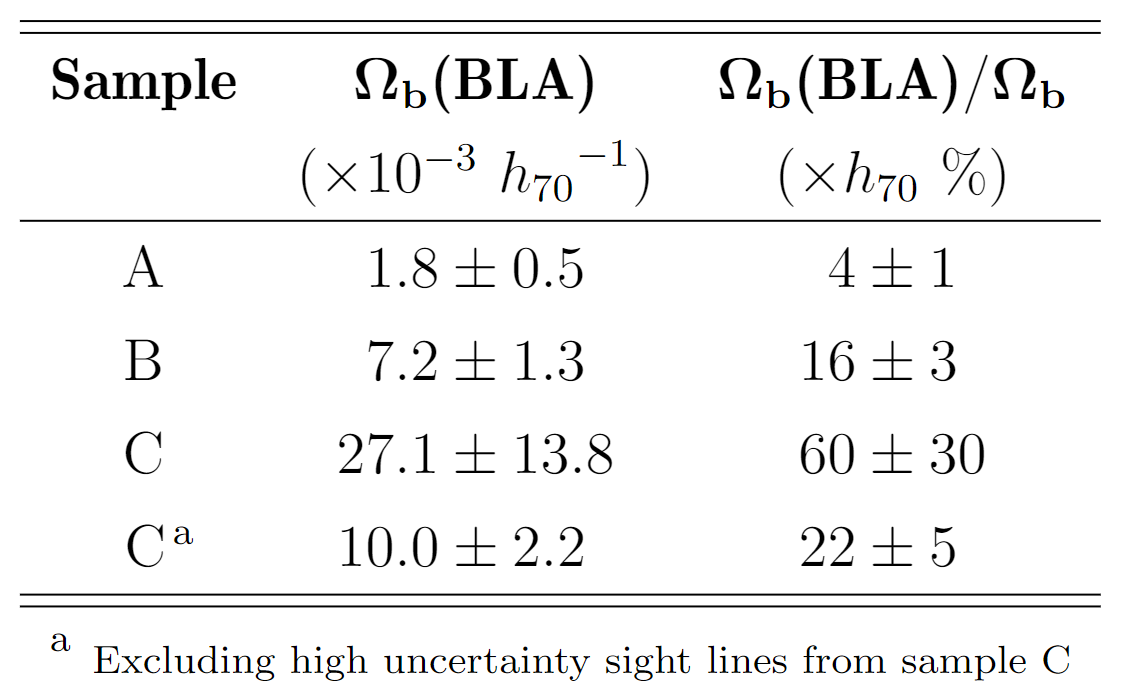
\includegraphics[width=7cm,draft=False]{Figures-Thesis/Omega-BLA-table.png}
            \end{figure}
          }
        \end{itemize} 

    
        \begin{tikzpicture}[remember picture, overlay,use page relative coordinates]
      
          \uncover<2->{\node at (0.23,0.14) {\footnotesize{Ref. : Planck Collaboration
          et al. (2020)}} ;}

          \uncover<4->{\draw[red, rounded corners, thick] (0.33,0.395) rectangle (0.7,0.455);}
          
        \end{tikzpicture}
    
        }
    
    
        
      \end{frame}
    
    